\chapter{Fejlesztési környezet és üzembe helyezés}

\section{Fejlesztői stack felállítása}
A fejlesztői környezet felállításához szükséges a \texttt{Docker}, \texttt{Docker Compose}, illetve a \texttt{make} eszköz telepítése. Ez a szakasz a Linux-alapú rendszerekre történő telepítést mutatja be. Windows esetén a WSL használata javasolt.

\begin{enumerate}
    \item \textbf{Repository klónozása:}
    \begin{verbatim}
git clone https://github.com/Csaba44/SkillIssue.git
cd SkillIssue
    \end{verbatim}

    \item \textbf{Környezeti változók létrehozása:}
    Másoljuk le a \texttt{.env.example} fájlt \texttt{.env} névvel, majd töltsük ki a \texttt{UID} és \texttt{GID} értékeket, amelyek a host felhasználó azonosítói. Ezek szükségesek a fájljogosultságok szinkronizálásához a konténer és a host között.
    \begin{verbatim}
cp .env.example .env
id -u && id -g
    \end{verbatim}

    Majd hasonlóan, másoljuk le a \texttt{.env.dev.example} fájlt \texttt{.env.dev} névvel:
    \begin{verbatim}
cp .env.dev.example .env.dev
    \end{verbatim}

    \item \textbf{Függőségek telepítése:}
    \begin{verbatim}
cd api && composer install
cd ../frontend && npm install
cd ../websocket && npm install
cd ..
    \end{verbatim}

    \item \textbf{Laravel alkalmazáskulcs generálása:}
    \begin{verbatim}
make dev-key
    \end{verbatim}
    A parancs kiír egy \texttt{base64:...} előtaggal kezdődő kulcsot, amelyet a \texttt{.env.dev} fájlban az \texttt{APP\_KEY} változóhoz kell rendelni.

    \item \textbf{Helyi host név hozzáadása:}
    A \texttt{/etc/hosts} fájlba fel kell venni a következő bejegyzést:
    \begin{verbatim}
127.0.0.1     skillissue.local
    \end{verbatim}
    WSL használata esetén a Windows host számítógépen a \texttt{C:/Windows/System32/drivers/etc/hosts} fájlba kell beleírni a fentebbi sort.
    \newpage
    \item \textbf{Fejlesztői stack elindítása:}
    \begin{verbatim}
make dev-up
    \end{verbatim}
    Az alkalmazás a \texttt{http://skillissue.local:5173} címen érhető el. A stack leállításához:
    \begin{verbatim}
make dev-down
    \end{verbatim}

    \item \textbf{Migrációk futtatása} (amennyiben nem futottak le automatikusan):
    \begin{verbatim}
make migrate-seed
    \end{verbatim}

\end{enumerate}

\begin{figure}[h]
    \centering
    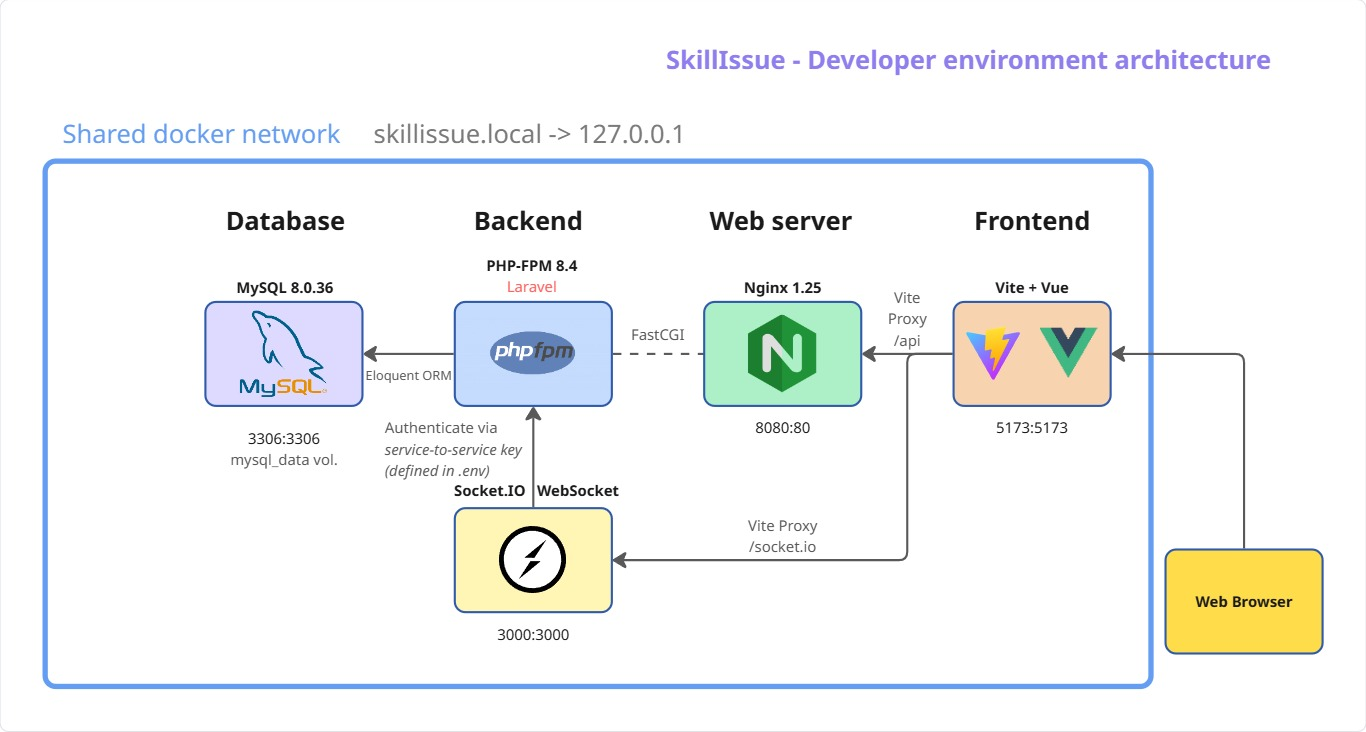
\includegraphics[width=\textwidth]{images/dev_diagram.png}
    \caption{A SkillIssue fejlesztői környezetének architektúrája}
    \label{fig:dev-architektura}
\end{figure}
\textbf{Megjegyzés:} Teszteléshez a SkillIssue weboldal is használható: https://skillissue.hu. Az alkalmazás jelszóval van védve:

\begin{center}
    \begin{tabular}{ll}
     \textbf{Felhasználónév} & skillissue \\
     \textbf{Jelszó} & neumanneger2026
    \end{tabular}
\end{center}

\section{Környezeti változók}
A környezeti változók három \texttt{.env} fájlban vannak tárolva:
\begin{description}
    \item[.env.dev] Fejlesztői környezet környezeti változói 
    \item[.env.prod] Éles környezet környezeti változói 
    \item[.env] A Dockerhez használatos környezeti változók, a jogosultság szinkronizálására a Docker konténer és a host számítógép között.
\end{description}
\newpage
\begin{center}
    \textit{Fontosabb Laravel környezeti változók}:\\
    \begin{tabular}{|c|l|}
        \hline
        \textbf{Környezeti változó neve} & \textbf{Leírás} \\
        \hline
        APP\_ENV & Lehetséges értéke: local, production. \\
        \hline
        APP\_KEY & Base64-el enkódolt kulcs, amit a Laravel alkalmazás titkosításra használ. \\
        \hline
        DB\_[*] & A Laravel által létrehozott adatbázis-kapcsolat paraméterei. \\
        \hline
        SESSION\_DRIVER & Pl.: cookie, database, file, stb. - Meghatározza, hol legyenek tárolva a session adatok. \\
        \hline
        SESSION\_LIFETIME & Session élettartama, percben. \\
        \hline
        SESSION\_ENCRYPT & Boolean, session adatok titkosított tárolása \\
        \hline
        SESSION\_PATH & A session cookie milyen URL-en legyen elérhető (/ = egész domain). \\
        \hline
        SESSION\_DOMAIN & Melyik domain-en legyen érvényes a session cookie. \\
        \hline
    \end{tabular}
\end{center}

\begin{center}
    \textit{Játékmenet és saját implementációkra vonatkozó környezeti változók:}\\
    \begin{tabular}{|c|l|}
        \hline
        \textbf{Környezeti változó neve} & \textbf{Leírás} \\
        \hline
        MAX\_ROUNDS & Hány körös legyen a mérkőzés (Solo és Ranked) \\
        \hline
        SOLO\_MAX\_GUESS\_TIME & Maximum válaszadási idő (másodperc, egyjátékos mód) \\
        \hline
        RANKED\_MAX\_GUESS\_TIME & Maximum válaszadási idő (másodperc, Ranked 1 vs. 1 mód) \\
        \hline
        SERVICE\_TOKEN & Service-to-service kommunikációhoz meghatározott közös token \\
        \hline
    \end{tabular}
\end{center}

A részletes dokumentáció megtalálható a \ref{ch:envvar} függelékben (Környezeti változók dokumentációja).

\section{Fejlesztői vs. Éles konfiguráció}
A konfigurációs különbségeket részletesen a \ref{sec:dockeconfig}. szakasz taglalja. 
\\
Összességében elmondható, hogy a \textbf{fejlesztői környezet} esetében az elsődleges szempont a könnyű elindítás, fejlesztés segítése, a hot-reload támogatása, parancssori eszközök (artisan) könnyű használatának biztosítása és a jogosultságok szinkronizálása. A fejlesztői környezetben az egységes munkavégzés érdekében \texttt{.prettierrc} Prettier konfigurációs fájl található, amely lehetővé teszi a kódbázis egységes formázását.
\\
Az \textbf{éles környezetben} a fő szempont az egyszerű szállítás, deployment, illetve a biztonság. 

\section{Makefile parancsok}
A hosszú parancsok kiküszöbölésének érdekében a Makefile segíti a fejlesztő munkáját. Hat részre van bontva: Dev, Migration, Build, Publish, Prod, Utils.
A Makefile összes utasítása és részletes leírása: \ref{ch:makefile} függelék (Makefile parancsok referencia)